\documentclass{article}
\usepackage{ctex}
\usepackage{amsmath}
\usepackage{amssymb}
\usepackage{minted}
\usepackage{graphicx}
\newcommand{\romannum}[1]{\uppercase\expandafter{\romannumeral#1}}
\setminted[C++]{autogobble,breaklines,fontsize=\footnotesize,mathescape}
\begin{document}
\title{Note on Dynamic Programming (\romannum{3})\\\large{Day 3 PM---Advanced Models}}\date{}\author{Hatsune Miku}
\maketitle
\section{Advanced Models}
\subsection{树模型}
\subsubsection{K-联通块}
N个点的树,点上有权值,求大小为K的联通块权值和的最大值。$K\le N\le 100.$

$f[i,j]$表示以$i$为根(包括i点),大小为$j$的联通块的权值和。
\begin{equation*}
    f[i,j]=\max\left\{\sum_{p=1}^kdp[ik,jp]\right\}+v_i
\end{equation*}
% TODO TikZ redraw.
\begin{figure}[h]
    \begin{center}
        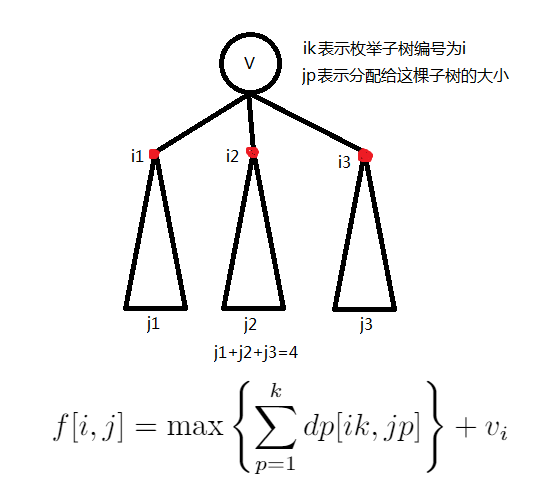
\includegraphics[width=5cm]{transtotikz.png}
    \end{center}
    \caption{对状态转移的解释}
    \label{fig. 1.1}
\end{figure}

转换成背包?有依赖的背包问题+泛化物品。假设现在有$j-1$块钱,对于每个孩子可以选择选和不选,选则增加收益,现在要求最大化收益。

所以本质上还是一个背包问题。要对背包问题形成敏感性,看到以上式子就应该考虑树上背包问题。
\subsection{外向树模型}
\subsubsection{直径}
\subsection{图论模型}
\subsubsection{等式}
\subsubsection{NOIP普及组初赛---载人过河}
\subsubsection{路径方案}
\subsection{状态压缩模型}

\subsubsection{棋盘上的王}
定义dp[i,j,s]表示前i行已经放了j个,并且前i行已经在s的集合中放了王。枚举集合$s'$为倒数第二行放的状态,且s与$s'$不互相攻击。
\begin{equation*}
    \begin{aligned}
        dp[i,j,s]=&\sum_{s'}dp[i,j-|s|,s']\\
        dp[i,j,s]\to& dp[i,j+|s|,s']
    \end{aligned}
\end{equation*}
状态压缩实际上是表示状态的一种技巧,可以将集合s转化成一个长度为n的01字符串,共有$2^n-1$中取值(状态压缩中的“压缩”对应将集合转化为一个数字)。

\begin{minted}{C++}
#include<cstdlib>
#include<cstring>
#include<cmath>
#include<cstdio>

const int Modulo = int(1e9+7);

void update(int &a,int &b) {
    a=(a % Modulo + b % Modulo) % Modulo;
}

int pop_count(int S) {
    int ans = 0;
    while(S) {
        if(S & 1) ans++;
        S >>= 1;
    }
    return ans;
}

bool is_valid(int S) {
    return ! bool(S & (S >> 1));
}

bool is_valid2(int S1,int S2) {
    return ! (bool(S1 & S2) || bool(S1 & (S2 >> 1)) || bool(S1 & (S2 << 1)));
}

int n,k,dp[11][101][1024];

int main(void) {
    scanf("%d%d", &n, &k);

    dp[0][0][0] = 1;
    for(int i = 1; i <= n; ++i) {
        for(int j = 0; j <= k; ++j) {
            for(int S = 0; S < (1 << n); ++S) if(is_valid(S)&&pop_count(S)<=j) {
                for(int SS = 0; SS < (1 << n); ++SS) if(is_valid(SS)) {
                    if(is_valid2(S, SS)) {
                        update(dp[i][j][S], dp[i-1][j-pop_count(S)][SS]);
                    }
                }
            }
        }
    }

    int ans = 0;
    for(int S = 0; S < (1 << n); ++S) if(is_valid(S)) {
            update(ans,dp[n][k][S]);
    }

    printf("%d",ans);
    return 0;
}
\end{minted}

\subsubsection{特殊序列}
\subsubsection{联通}
\subsection{数位模型}
\subsubsection{数位翻转}
\subsubsection{翻转求和}
\subsubsection{组合数计数(BZOJ4737)}
\end{document}
